\documentclass{article}
\usepackage[utf8]{inputenc}
\usepackage[spanish]{babel}
\usepackage{listings}
\usepackage{graphicx}
\graphicspath{ {images/} }
\usepackage{cite}

\begin{document}

\begin{titlepage}
    \begin{center}
        \vspace*{1cm}
            
        \Huge
        \textbf{Proyecto de investigación}
            
        \vspace{0.5cm}
        \LARGE
        Nociones de la memoria del computador
            
        \vspace{1.5cm}
            
        \textbf{Oscar Andrés Gutiérrez Rivadeneira}
            
        \vfill
            
        \vspace{0.8cm}
            
        \LARGE
        Departamento de Ingeniería Electrónica y Telecomunicaciones\\
        Universidad de Antioquia\\
        Medellín\\
        Septiembre de 2020
            
    \end{center}
\end{titlepage}

\tableofcontents

\newpage

\section{Introducción} 
Al referirnos a la memoria no podemos evitar pensar en un computador, pero muchos son muchos los que desconocen que este componente electrónico esta presente en muchos más dispositivos, entre los cuales se encuentran: los celulares, tabletas, televisores, consolas de juego, entre otros. Siendo así la memoria un componente de suma importancia para el funcionamiento de nuestros dispositivos, llegando al punto en el que sin la memoria el dispositivo no puede ni tan siquiera arrancar, procesar datos, ejecutar instrucciones y demás.\cite{tipos-memoria}

Además, hay distintos tipos de memoria, aunque en esencia todas hacen lo mismo, almacenar, todas lo hacen de manera distinta, con un objetivo distinto, con diferente capacidad y velocidad.\hfill
\vspace{4mm}

Ahora bien, si existe una gran variedad de dispositivos que utilizan los diferentes tipos de memoria, en este documento vamos a enfocarnos en la memoria del computador, dando solución a las preguntas planteadas en el taller "nociones de la memoria del computador".

\section{¿Que es la memoria de un computador?} \label{contenido}
La memoria es un componente que se encarga retener, memorizar o almacenar datos durante un periodo de tiempo.\cite{definicion}
Siendo así, un componente con un papel muy importante, desde el momento en el que se enciende el computador, hasta el momento en que se apaga, la memoria se encuentra activa (o bien sea las memoras, teniendo en cuenta que no solo existe un tipo de memoria y que no hay solo una por computador) permitiendo que el microprocesador pueda acceder a los datos que requiere para gestionar la computadora y permitir así que el usuario tenga a acceso a los diversos archivos y aplicaciones que tenga almacenados. A continuación se muestra una memoria RAM, siendo esta la más conocida y la que primero nos suele venir a la mente a la hora de hablar sobre memorias. Figura \ref{fig:memoriapc}

\begin{figure}[h]
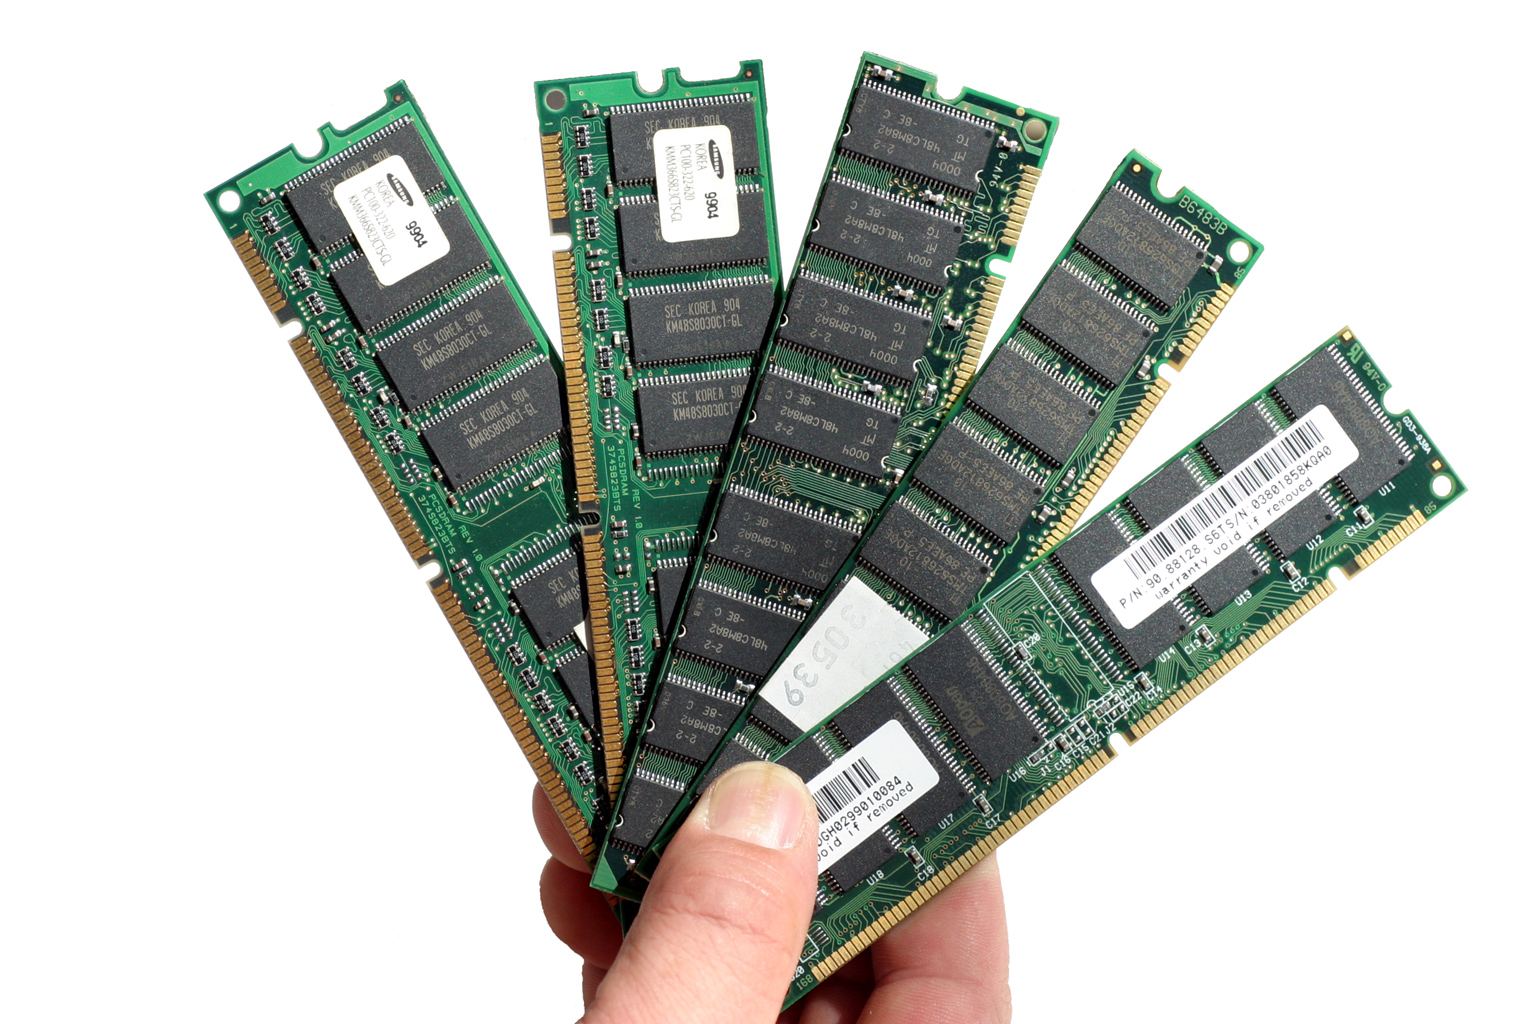
\includegraphics[width=7cm]{Memoria.jpg}
\centering
\caption{Memoria RAM de un pc}
\label{fig:memoriapc}
\end{figure}


\section{Tipos de memoria} \label{contenido}
Como se ha comentado no existe solo un tipo de memoria, sino que son varios tipos de memoria, los cuales actúan en situaciones diferentes, a velocidades diferentes y además, tiene capacidades diferentes; a pesar de que todas tienen la función de almacenar información. 
Entre los tipos de memoria mas comunes tenemos:
\begin{enumerate}
\item \textbf{Memoria caché:} <<La memoria cache nació cuando se descubrió que las memorias ya no eran capaces de acompañar a la velocidad del procesador>> \cite{tipos-memoria}, lo cual provocaba retrasos en el procesador el cual debía quedar esperando a que la memoria RAM entregase los datos para así poderlos procesar. La solución a este problema fue crear un tipo de memoria ultra-rápida que fuese capaz de almacenar los datos que el procesador requiere con mayor frecuencia para impedir estos retrasos.
Aunque este aumento significativo en la velocidad de la memoria suponía un problema, y es que este tipo de memoria son muy costosas, lo cual haría que un computador hogareño fuese algo casi imposible de adquirir, la solución a este nuevo problema sería usar la memoria cache en menos cantidades y poder colocar así otro tipo de memorias que, aunque más lentas, son más económicas y tienen mayor capacidad de almacenamiento. 
Este tipo de memoria, a su vez esta dividida en tres tipos o como se les llama, niveles, los cuales son:
\subitem L1(Nivel 1): Esta se encuentra dentro de los núcleos de procesador, funcionando a la misma velocidad de estos pero con una capacidad individual en promedio de 32kilo-bytes.
\subitem L2(Nivel 2): También se encuentras dentro de los núcleos pero siendo estas un poco más lentas, aunque con mayor capacidad, teniendo en promedio una capacidad individual de almacenar 256kilo-bytes.
\subitem L3(Nivel 3): Se encuentra dentro del procesador, pero por fuera de los núcleos, por lo que es compartida por todos. Es más lenta pero posee más capacidad que las anteriores, en promedio 12Mega-bytes. 
    \begin{figure}[h]
        \centering
        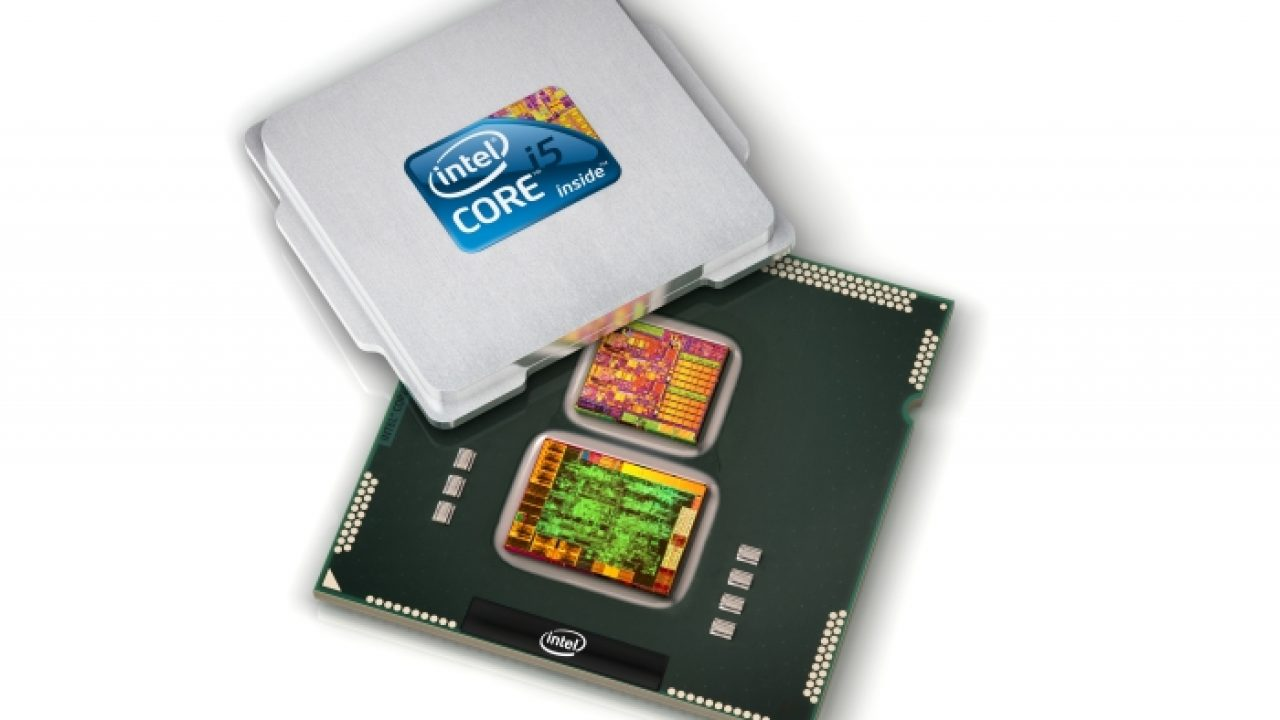
\includegraphics[scale=0.25]{Memoria cache.jpg}
        \caption{Memoria cache}
        \label{fig:memoriacachel}
    \end{figure}


\item \textbf{Memoria RAM}: Considerada la memoria más importante del computador, la memoria RAM o Random Access Memory, posee menos velocidad que la memoria caché, pero podemos tener mucha RAM a un precio bastante asequible, por lo que la mayor parte de los datos se almacena en esta; no obstante, debemos tener en cuenta de que es volátil, lo que quiere decir que todos los datos que fueron cargados en ella se perderán cuando el computador se apague.
    \begin{figure}[h]
        \centering
        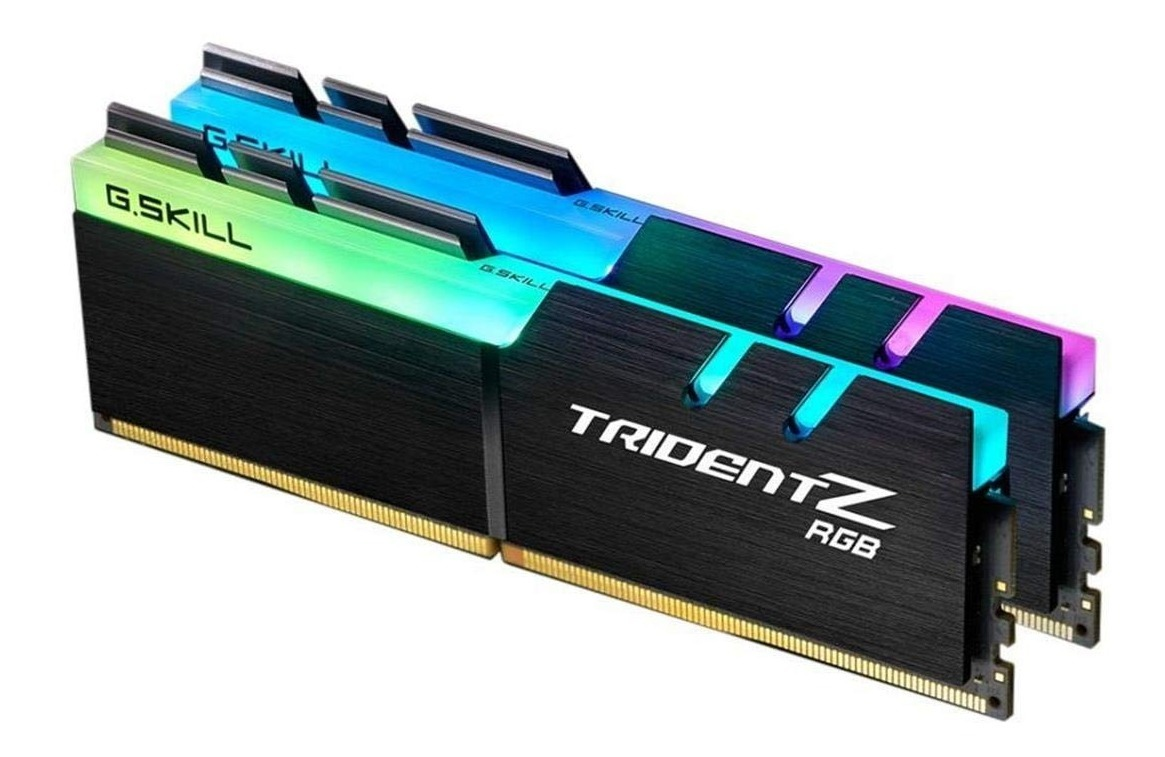
\includegraphics[width=8cm]{Memoria RAM.jpg}
        \caption{Memoria RAM}
        \label{fig:memoriaram}
    \end{figure}
    
\item \textbf{Memoria ROM:} Se encuentra de fabrica en la placa madre, y contiene la información que requiere el computador a la hora de encender. Debido a la importancia de los datos que contiene no puede ser alterada por el usuario mediante aplicaciones, de ahí su nombre ROM(Read Only Memory); además no es volátil, lo que quiere decir que sus datos permanecen aun cuando se apaga el computador. \cite{tecnología-informática}
    \begin{figure}[h]
        \centering
        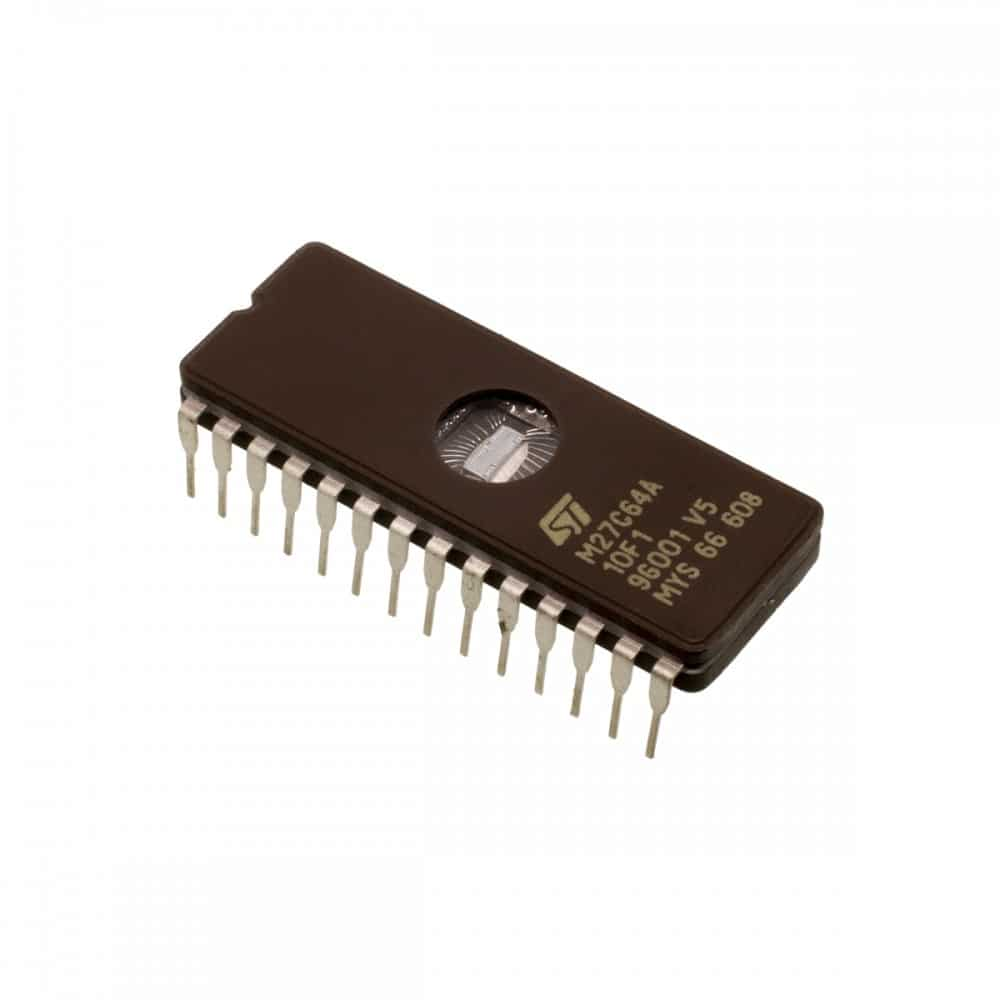
\includegraphics[scale=0.15]{Memoria ROM.jpg}
        \caption{Memoria ROM}
        \label{fig:memoria_rom}
    \end{figure}

\item \textbf{Memoria Virtual:} Se trata una una parte del disco duro que se encuentra dedicada para almacenar ciertas partes de las aplicaciones que no se van a utilizar, evitando que ocupen espacio innecesario en la memoria, dejando así disponibilidad para que otros programas se puedan ejecutar y sean almacenados en la memoria RAM, mientras tanto los datos que se encuentran en la memoria virtual están listos para cuando el usuario quiera acceder a ellos.

\item \textbf{Disco Duro:} Son dispositivos no volátiles (que su información se mantiene aún luego de apagar el computador) encargados de retener la información del usuario. Fotografías, vídeos, archivos de texto, programas, e incluso, el sistema operativo.\cite{qloudea}
    \begin{figure}[h]
        \centering
        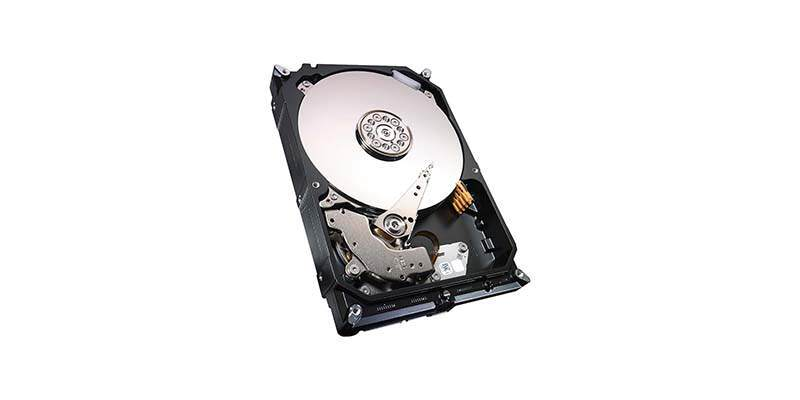
\includegraphics[width=10cm]{Disco Duro.jpg}
        \caption{Disco Duro}
        \label{fig:my_label}
    \end{figure}
\end{enumerate}

\section{¿Cómo las distintas memorias gestionan el computador?} \label{contenido}
Mucho se ha hablado acerca de la importancia de los distintos tipos de memoria para el computador, sus funciones, entre otros. Pero, ¿cómo comienzan a operar las memorias desde el momento en que se enciende un computador?
\begin{itemize}

\item Una vez se enciende el computador, el microprocesador necesita programas para funcionar, por lo que primero toma desde la ROM su primera instrucción llamada POST (Power-On-Self-Test), la cual le indica que realice un chequeo de todos los componentes necesarios para arrancar.

\item Luego se carga en la RAM un programa llamado BIOS (Basic Input Output System), el cual contiene información sobre todos los componentes del equipo, permitiendo que cuando el microprocesador necesite recibir o enviar información a estos componentes solo busca su dirección, la cual fue previamente cargada en la RAM

\item Ahora que el microprocesador tiene las instrucciones suficientes, carga el sistema operativo en la RAM y lo mantiene ahí hasta que se apague el computador, ya que el microprocesador hará uso de este en todo momento, por lo que necesita acceso inmediato a el.

\item Ya con el sistema operativo cargado podemos comenzar a trabajar con nuestros programas y aplicaciones. Pero para no utilizar toda la memoria solo se cargan las partes esenciales, dejando las otras partes de los programas en la memoria virtual para luego cargarlos en la RAM cuando sea necesario.

\item A la hora de cerrar una aplicación, si se guardan los cambios, éstos se almacenan en el disco duro y la aplicación y el archivo son quitados de la RAM

\end{itemize}

\section{}

\section{Conclusión} \label{conclulsion}

\bibliographystyle{IEEEtran}
\bibliography{references}

\end{document}
